\documentclass{scrartcl}
\usepackage[T1]{fontenc}

% u/ masukin gambar
\usepackage{graphicx}

% u/ bikin ornament

% u/ mengatur margin kertas
\usepackage{geometry}
\geometry{
	a4paper,
	left=3.5cm,
	right=2.5cm,
	bottom=2.5cm,
	top=3cm
}

% u/ referensi
\usepackage{hyperref}

% u/ bikin tabel
\usepackage{tabu}
\usepackage{booktabs}

% u/ masukin source code
\usepackage{minted}
\usemintedstyle{vs}
\setminted[]{
	breaklines=true,
	tabsize=2,
	autogobble=true
}

% Content -> Daftar Isi
\renewcommand{\contentsname}{Daftar Isi}

\begin{document}
	
	% kop judul handout
	\begin{center}
		\begin{tabu} to \linewidth {X[c]}
			\toprule
			\\
			\LARGE{\textbf{Handout Praktikum Mobile Application}} \\
			\\
			\large{Topik 1 -- Activity dan Intent} \\
			\\
			\bottomrule
		\end{tabu}
	\end{center}
	
	\tableofcontents
	
	\section{Tujuan}
	
	\begin{enumerate}
		\item Mahasiswa dapat mengetahui cara menyimpan data sederhana menggunakan obyek \texttt{SharedPreferences}
		\item Mahasiswa dapat mengetahui cara memperbolehkan pengguna untuk memodifikasi preferensi menggunakan kelas \texttt{PreferenceActivity}
		\item Mahasiswa dapat mengetahui cara menulis dan membaca file dari penyimpanan internal dan eksternal
		\item Mahasiswa dapat mengetahui cara membuat dan menggunakan basis data SQLite
	\end{enumerate}
	
	\section{Komponen/Peralatan}
	
	\begin{itemize}
		\item PC/laptop
		\item Android Studio
	\end{itemize}
	
	\section{Dasar Teori}
	
	\section{Langkah Praktikum}
	
	\subsection{Menyimpan Data Menggunakan Obyek \texttt{SharedPreferences}}
	
	\begin{enumerate}
		\item Buat proyek baru dengan nama \textbf{UsingPreferences} (opsi yang lain dibiarkan \textit{default}).
		
		\item Buat file baru dengan nama \texttt{myapppreferences.xml}, lalu taruh di direktori \\ \texttt{app/res/xml/}.
		
		\item Buka \texttt{myapppreferences.xml}, lalu \textit{copy-paste} listing di bawah ini.
		
		\begin{minted}{xml}
		<?xml version="1.0" encoding="utf-8"?>
		<PreferenceScreen
			xmlns:android="http://schemas.android.com/apk/res/android">
			<PreferenceCategory android:title="Category 1">
				<CheckBoxPreference
					android:title="Checkbox"
					android:defaultValue="false"
					android:summary="True or False"
					android:key="checkboxPref" />
			</PreferenceCategory>
			<PreferenceCategory android:title="Category 2">
				<EditTextPreference
					android:hint="[Enter a string here]"
					android:summary="Enter a string"
					android:title="Edit Text"
					android:key="editTextPref" />
				<RingtonePreference
					android:summary="Select a ringtone"
					android:title="Ringtones"
					android:key="ringtonePref" />
				<PreferenceScreen
					android:title="Second Preference Screen"
					android:summary=
					"Click here to go to the second Preference Screen"
					android:key="secondPrefScreenPref" >
					<EditTextPreference
					android:hint="[Enter a string here]"
					android:summary="Enter a string"
					android:title="Edit Text (second Screen)"
					android:key="secondEditTextPref" />
				</PreferenceScreen>
			</PreferenceCategory>
		</PreferenceScreen>
		\end{minted}
		
		\item Buat file baru dengan nama \texttt{prefheaders.xml}, lalu taruh di direktori \texttt{app/res/xml/}
		
		\item Buka \texttt{prefheaders.xml} lalu \textit{copy-paste} listing berikut ini.
		
		\begin{minted}{xml}
		<?xml version="1.0" encoding="utf-8"?>
		<preference-headers
			xmlns:android="http://schemas.android.com/apk/res/android">
			<header android:fragment= 
				"com.example.usingpreferences.AppPreferenceActivity$PrefFragment"
				android:title="Preferences"
				android:summary="Sample preferences" />
		</preference-headers>
		\end{minted}
		
		\item Buat file baru dengan nama \texttt{AppPreferenceActivity.java}, lalu taruh di direktori \texttt{app/java/com.example.usingpreferences}
		
		\item Buka file \texttt{AppPreferenceActivity.java}, lalu \textit{copy-paste} listing berikut ini.
		
		\begin{minted}{java}
		package com.example.usingpreferences;
		
		import android.os.Bundle;
		import android.preference.PreferenceActivity;
		import android.preference.PreferenceFragment;
		import android.preference.PreferenceManager;
		
		import java.util.List;
		
		public class AppPreferenceActivity extends PreferenceActivity {
		
			@Override
			public void onCreate(Bundle savedInstanceState) {
				super.onCreate(savedInstanceState);
			}
			
			@Override
			public void onBuildHeaders(List<Header> target) {
				loadHeadersFromResource(R.xml.prefheaders, target);
			}
			
			@Override
				protected boolean isValidFragment(String fragmentName) {
				return true;
			}
			
			public static class PrefFragment extends   PreferenceFragment {
				@Override
				public void onCreate(Bundle savedInstanceState) {
					super.onCreate(savedInstanceState);
			
					PreferenceManager.setDefaultValues(getActivity(),
					R.xml.myapppreferences, false);
			
					// load the preferences from an XML resource
					addPreferencesFromResource(R.xml.myapppreferences);
				}
			}
		}
		\end{minted}
		
		\item Buka \texttt{AndroidManifest.xml}, lalu \textit{copy-paste} listing berikut ini.
		
		\begin{minted}{xml}
		<?xml version="1.0" encoding="utf-8"?>
		<manifest xmlns:android="http://schemas.android.com/apk/res/android"
			package="com.example.usingpreferences">
			
			<application
				android:allowBackup="true"
				android:icon="@mipmap/ic_launcher"
				android:label="@string/app_name"
				android:roundIcon="@mipmap/ic_launcher_round"
				android:supportsRtl="true"
				android:theme="@style/AppTheme">
				<activity android:name=".MainActivity">
					<intent-filter>
						<action android:name="android.intent.action.MAIN" />
						<category android:name="android.intent.category.LAUNCHER" />
					</intent-filter>
				</activity>
				<activity
					android:name=".AppPreferenceActivity"
					android:label="@string/app_name" >
					<intent-filter>
						<action android:name="com.example.AppPreferenceActivity" />
						<category android:name="android.intent.category.DEFAULT" />
					</intent-filter>
				</activity>
			</application>
		
		</manifest>
		\end{minted}
		
		\item Buka \texttt{activity\_main.xml}, lalu \textit{copy-paste} listing berikut ini.
		
		\begin{minted}{xml}
		<?xml version="1.0" encoding="utf-8"?>
		<android.support.constraint.ConstraintLayout xmlns:android="http://schemas.android.com/apk/res/android"
			xmlns:app="http://schemas.android.com/apk/res-auto"
			xmlns:tools="http://schemas.android.com/tools"
			android:id="@+id/activity_main"
			android:layout_width="match_parent"
			android:layout_height="match_parent"
			tools:context="com.example.usingpreferences.MainActivity">
			
			<Button
				android:text="Load Preferences Screen"
				android:layout_width="310dp"
				android:layout_height="wrap_content"
				android:id="@+id/btnPreferences"
				app:layout_constraintLeft_toLeftOf="@+id/activity_main"
				android:layout_marginStart="16dp"
				app:layout_constraintTop_toTopOf="@+id/activity_main"
				android:layout_marginTop="16dp"
				app:layout_constraintRight_toRightOf="@+id/activity_main"
				android:layout_marginEnd="16dp"
				app:layout_constraintBottom_toBottomOf="@+id/activity_main"
				android:layout_marginBottom="16dp"
				app:layout_constraintVertical_bias="0.0"
				android:onClick="onClickLoad"
				android:layout_marginRight="40dp"
				android:layout_marginLeft="40dp" />
			<Button
				android:text="Display Preferences Values"
				android:layout_width="310dp"
				android:layout_height="wrap_content"
				android:id="@+id/btnDisplayValues"
				app:layout_constraintLeft_toLeftOf="@+id/btnPreferences"
				app:layout_constraintTop_toBottomOf="@+id/btnPreferences"
				android:layout_marginTop="16dp"
				app:layout_constraintRight_toRightOf="@+id/btnPreferences"
				android:onClick="onClickDisplay"/>
			<EditText
				android:layout_width="310dp"
				android:layout_height="wrap_content"
				android:inputType="textPersonName"
				android:ems="10"
				android:id="@+id/editText"
				app:layout_constraintLeft_toLeftOf="@+id/btnPreferences"
				app:layout_constraintTop_toBottomOf="@+id/btnDisplayValues"
				android:layout_marginTop="16dp"
				app:layout_constraintRight_toRightOf="@+id/btnPreferences" />
			<Button
				android:text="Modify Preferences Values"
				android:layout_width="fill_parent"
				android:layout_height="wrap_content"
				android:id="@+id/btnModifyValues"
				app:layout_constraintLeft_toLeftOf="@+id/btnDisplayValues"
				app:layout_constraintTop_toBottomOf="@+id/editText"
				android:layout_marginTop="16dp"
				app:layout_constraintRight_toRightOf="@+id/btnDisplayValues"
				android:onClick="onClickModify" />
		
		</android.support.constraint.ConstraintLayout>
		\end{minted}
		
		\item Buka \texttt{MainActivity.java}, lalu \textit{copy-paste} listing berikut ini.
		
		\begin{minted}{java}
		package com.example.usingpreferences;
		
		import android.content.Intent;
		import android.os.Bundle;
		import android.support.v7.app.AppCompatActivity;
		import android.view.View;
		
		public class MainActivity extends AppCompatActivity {
		
			@Override
			protected void onCreate(Bundle savedInstanceState) {
				super.onCreate(savedInstanceState);
				setContentView(R.layout.activity_main);
			}
			
			public void onClickDisplay(View view) {
			}
			
			public void onClickModify(View view) {
			}
			
			public void onClickLoad(View view) {
				Intent i = new Intent("com.example.AppPreferenceActivity");
				startActivity(i);
			}
		}
		
		\end{minted}
		
		\item Tekan \texttt{Shift + F9} (atau pilih \texttt{Run > Debug}) untuk men-\textit{debug} aplikasi. Pilih salah satu Android Virtual Device yang kalian inginkan.
		
		\item Pilih \texttt{LOAD PREFERENCES SCREEN} untuk melihat layar Preference Header. Hasil akhir ditunjukkan pada Figur \ref{fig:screenshot_1497490686}
		
		\item Pilih \texttt{Preferences} untuk melihat layar Preferences, lalu atur preferensi sesuai keinginan. Sebagai contoh bisa dilihat pada figur \ref{fig:screenshot_1497490676}, \ref{fig:screenshot_1497490686}, \ref{fig:screenshot_1497490697}.
		
		\item Klik tombol Home, lalu jalankan lagi aplikasi-nya. Kalian perhatikan bahwa preferensi yang kalian sudah atur tidak berubah.
		
		\begin{figure}[htbp]
			\begin{minipage}{.5\textwidth}
				\centering
				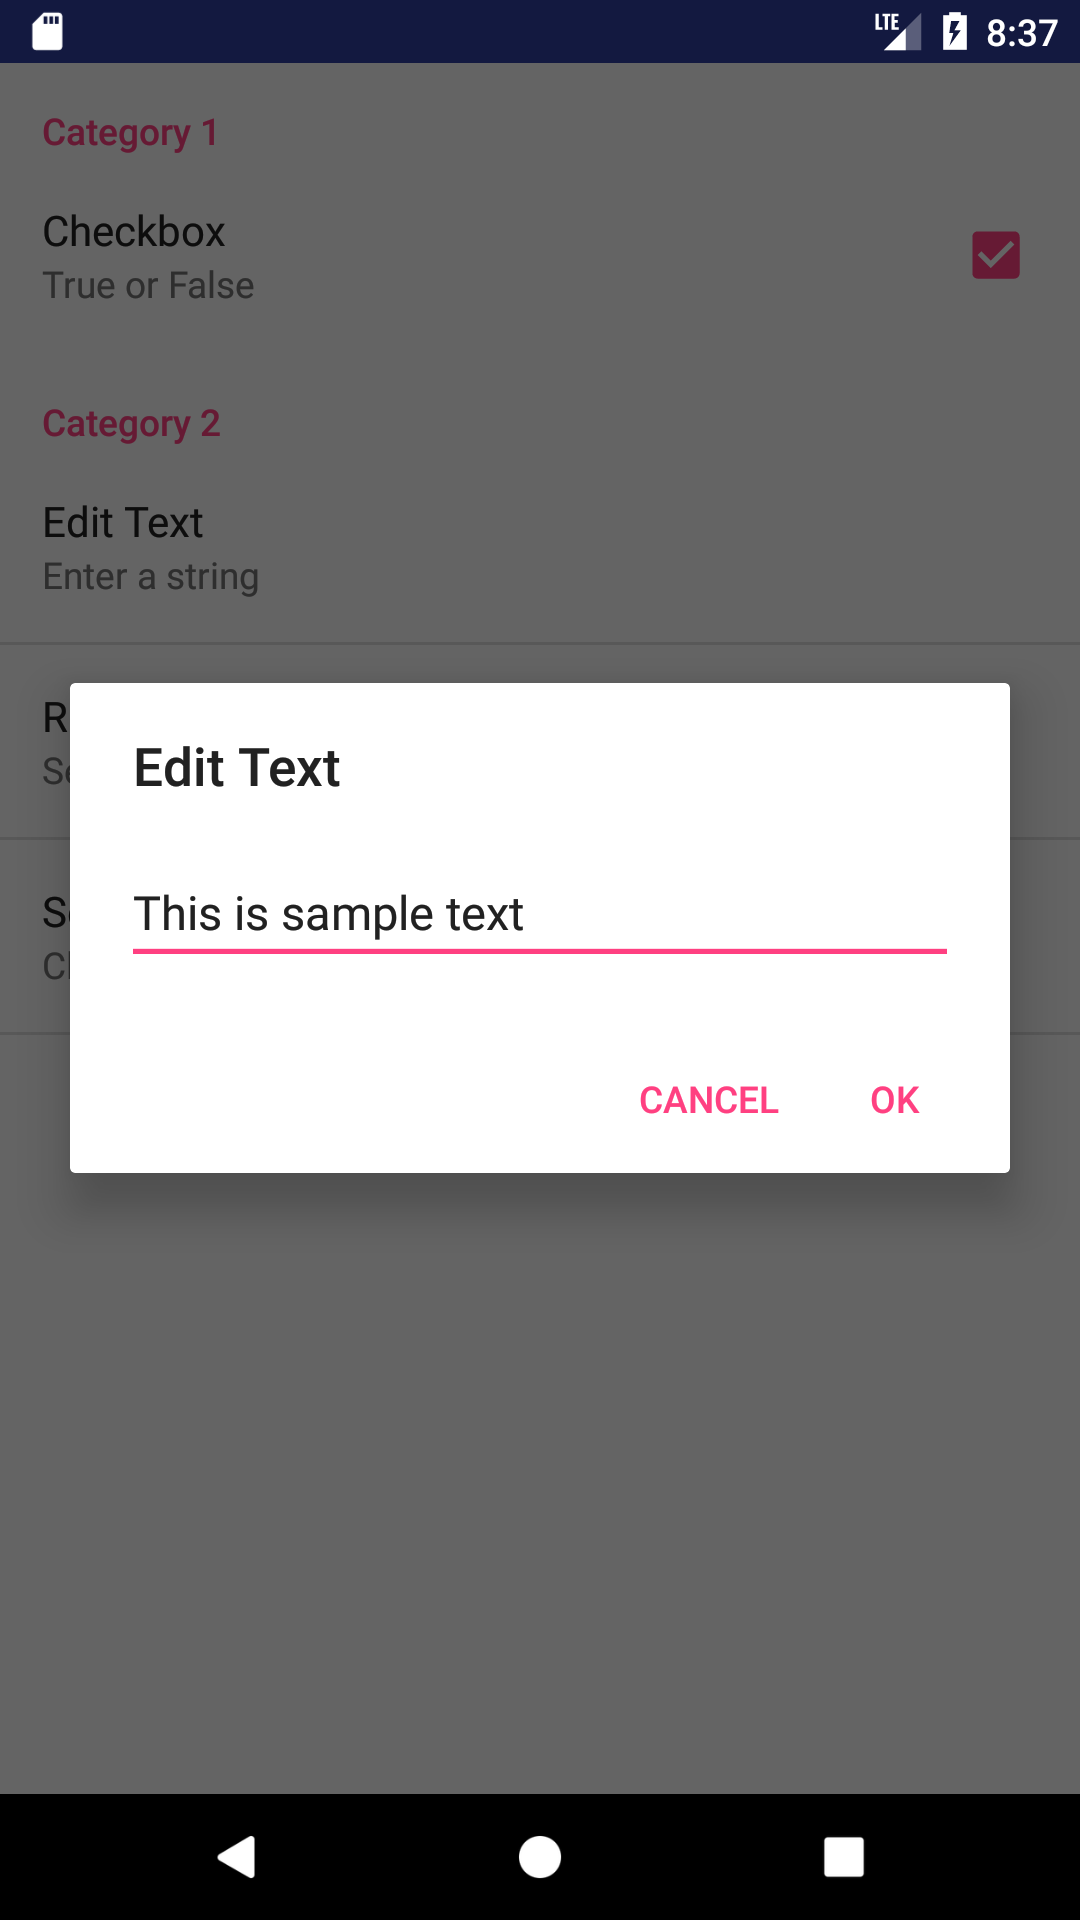
\includegraphics[width=0.7\linewidth]{Screenshot_1497490676}
				\caption{Hasil Akhir (1)}
				\label{fig:screenshot_1497490676}
			\end{minipage}%
			\begin{minipage}{.5\textwidth}
				\centering
				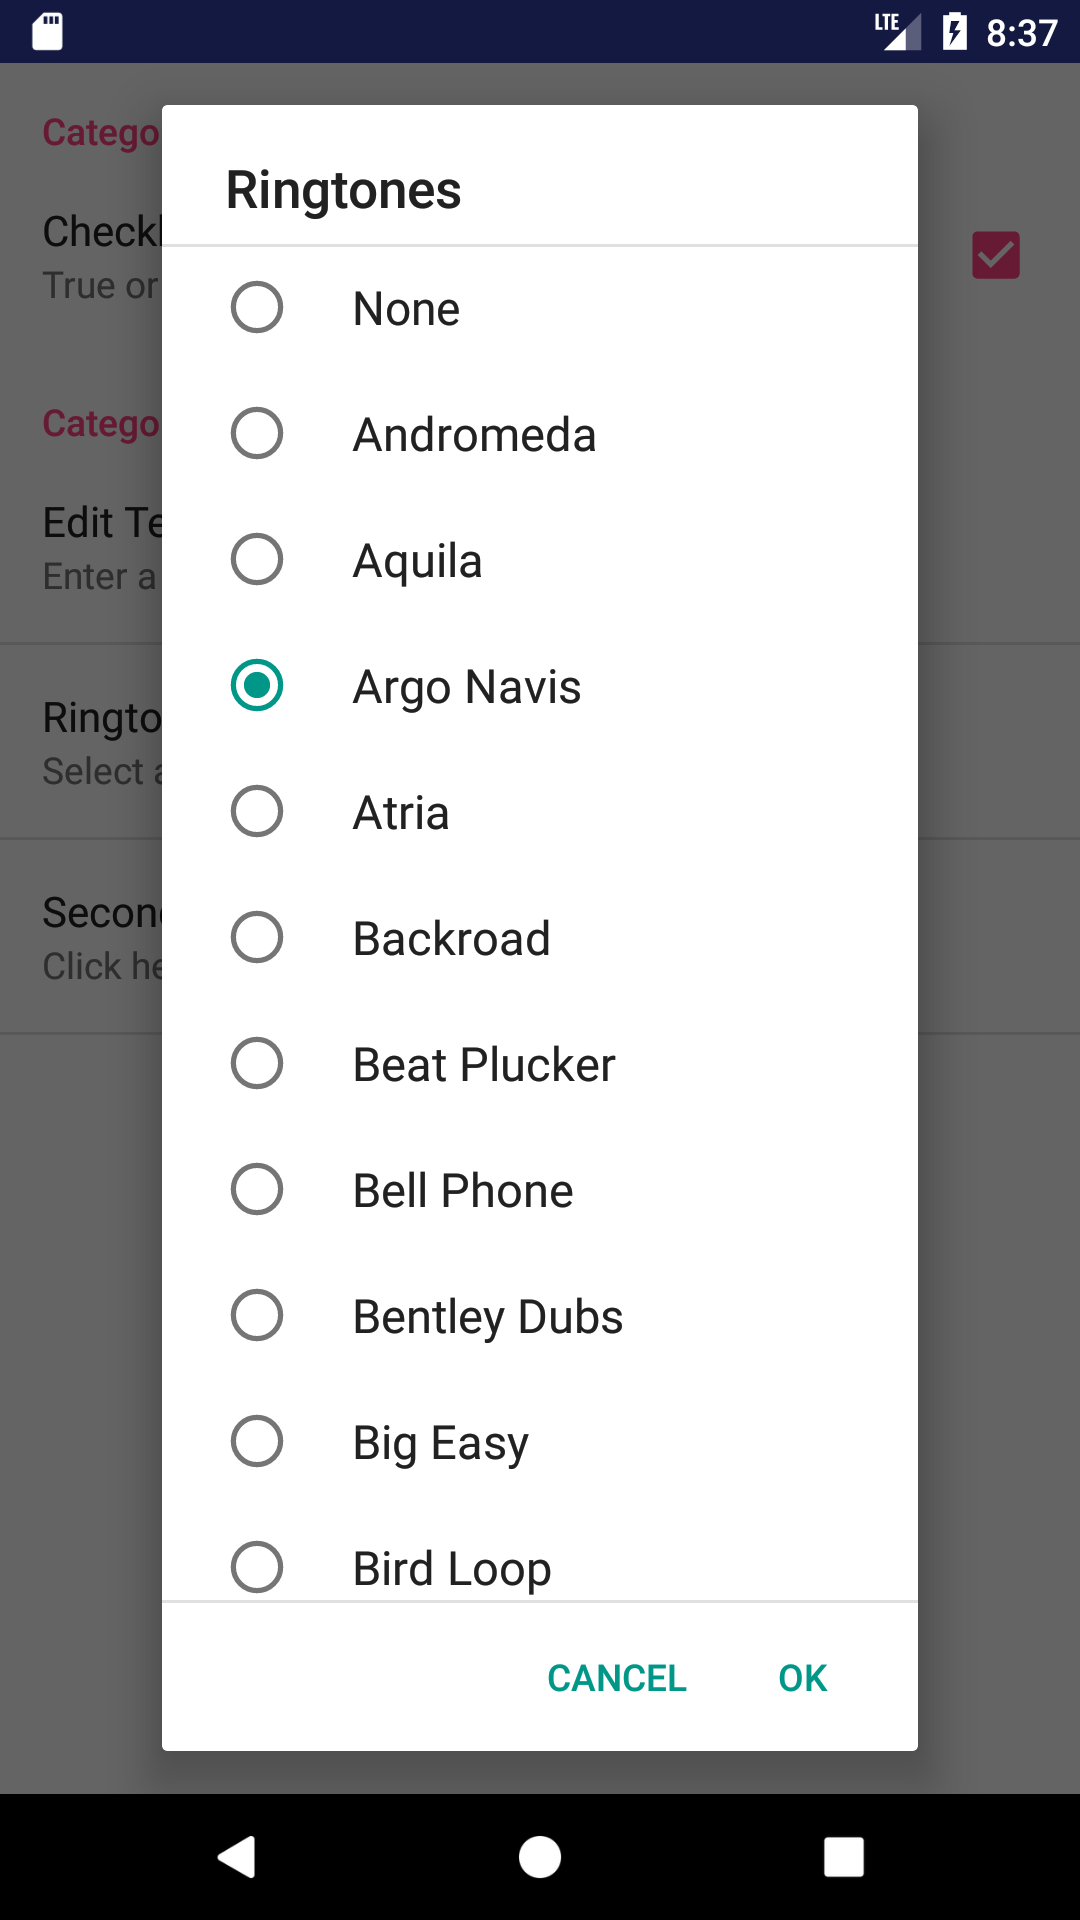
\includegraphics[width=0.7\linewidth]{Screenshot_1497490686}
				\caption{Hasil Akhir (2)}
				\label{fig:screenshot_1497490686}
			\end{minipage}
		\end{figure}
	
		\begin{figure}[htbp]
			\begin{minipage}{.5\textwidth}
				\centering
				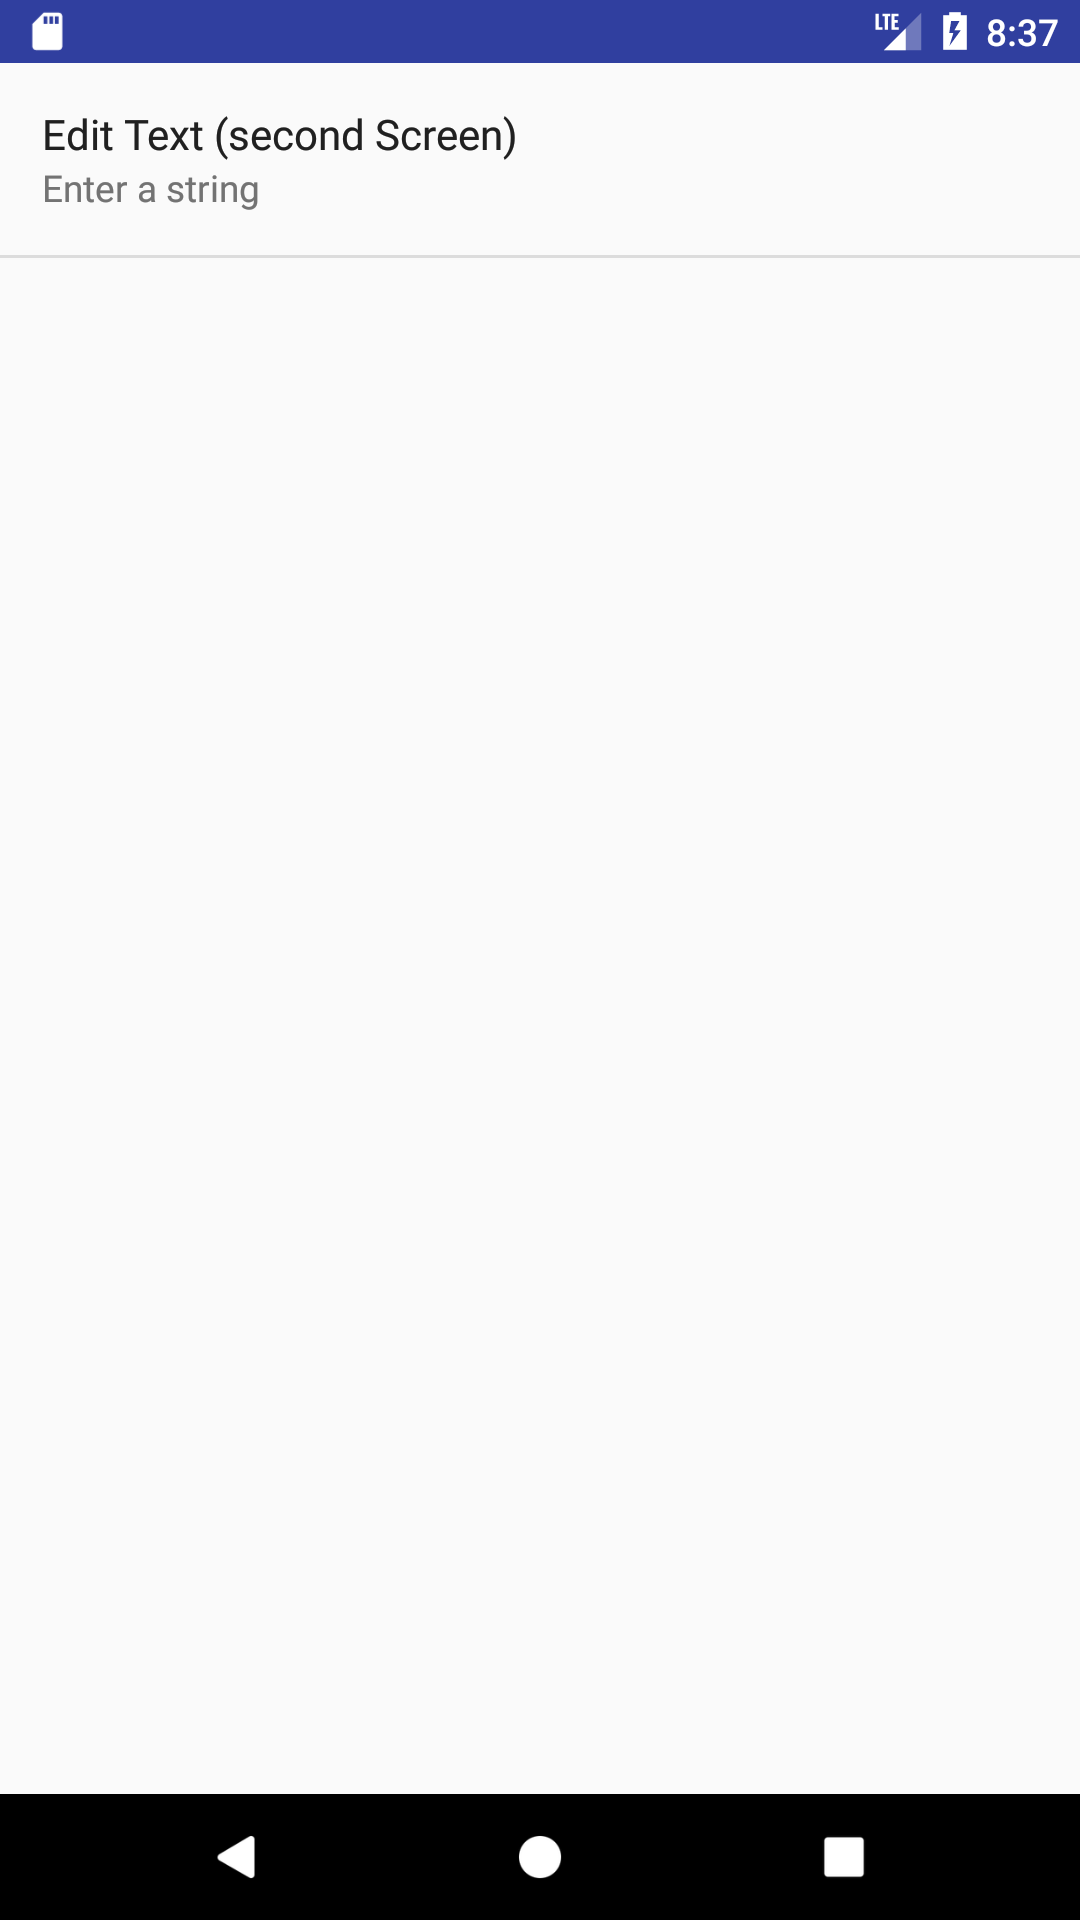
\includegraphics[width=0.7\linewidth]{Screenshot_1497490697}
				\caption{Hasil Akhir (3)}
				\label{fig:screenshot_1497490697}
			\end{minipage}%
			\begin{minipage}{.5\textwidth}
				\centering
				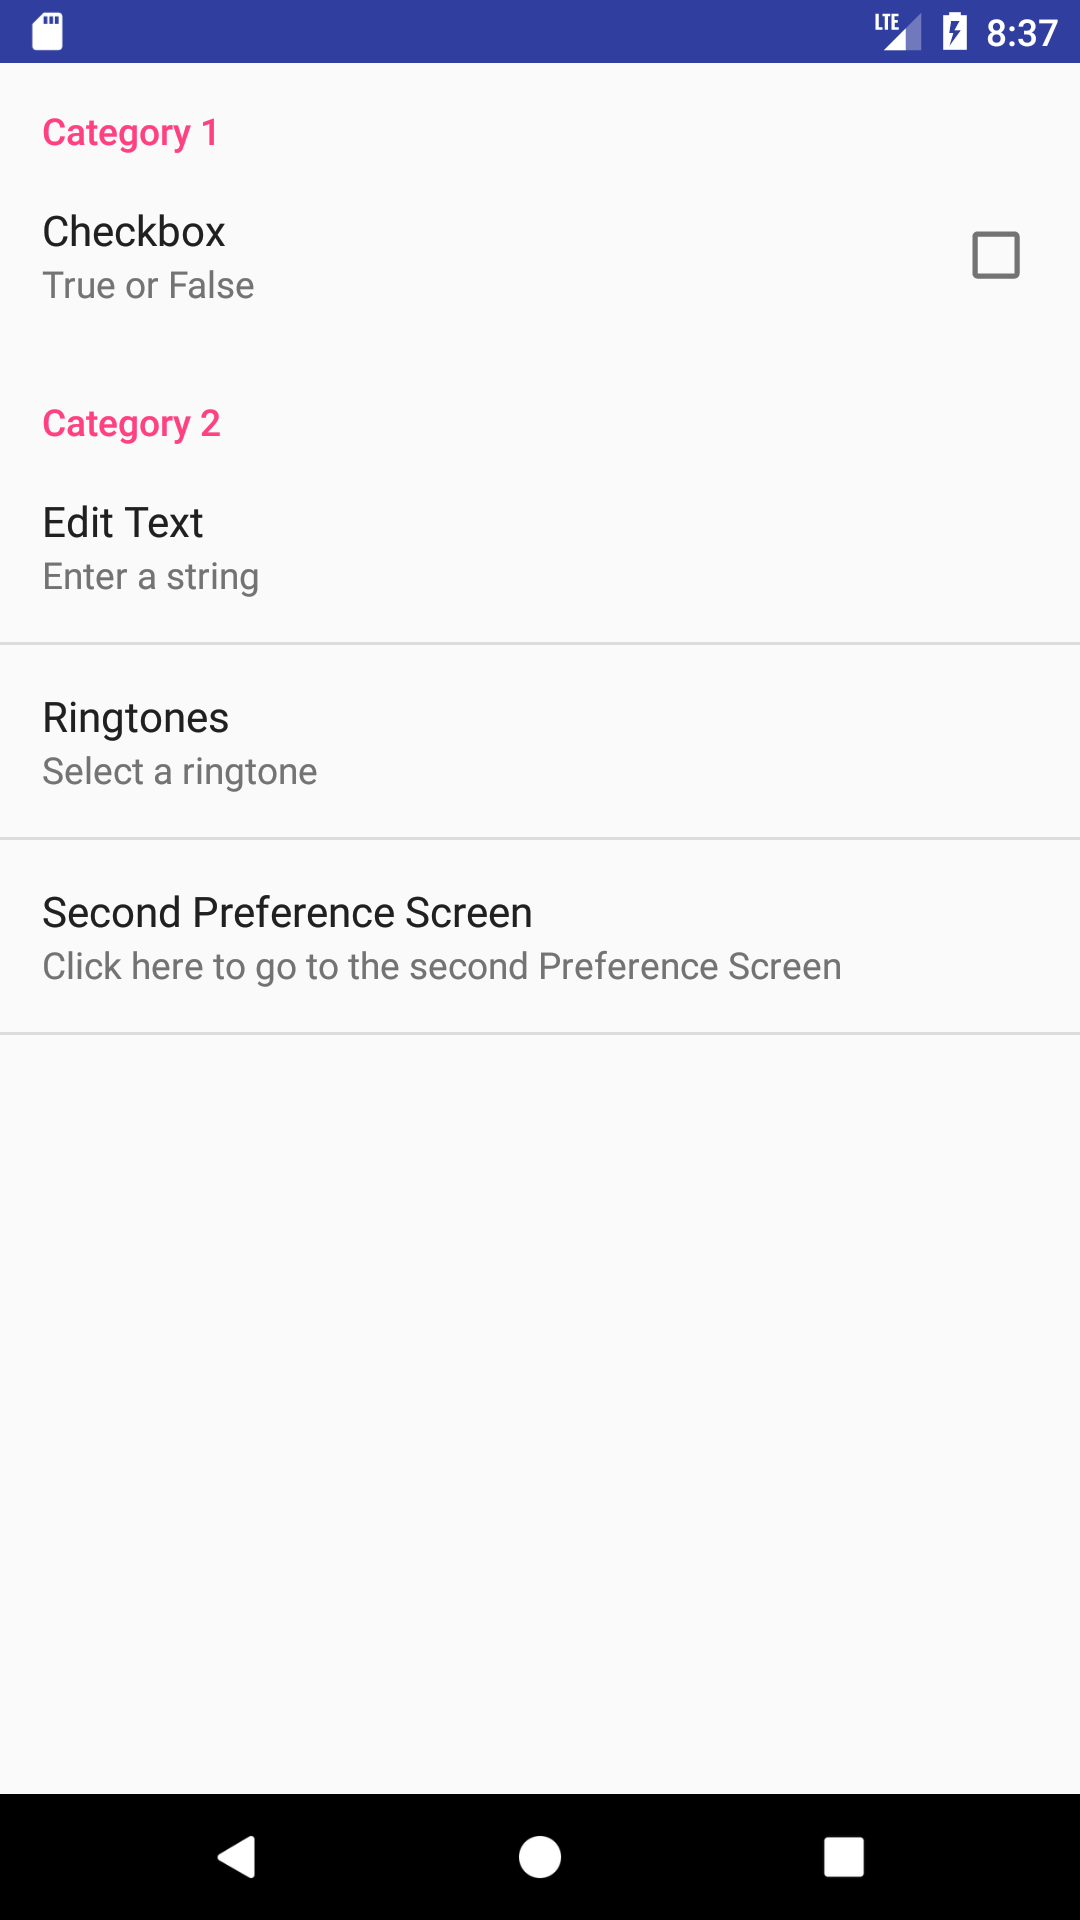
\includegraphics[width=0.7\linewidth]{Screenshot_1497490644}
				\caption{Hasil Akhir (4)}
				\label{fig:screenshot_1497490644}
			\end{minipage}
		\end{figure}
		
	\end{enumerate}

	\subsection{Mengambil dan Memodifikasi Preferensi}
	
	\begin{enumerate}
		\item Gunakan kembali proyek \texttt{SharedPreferences}.
		\item Buka \texttt{MainActivity.java}, lalu \textit{copy-paste} listing berikut ini.
		
		\begin{minted}{java}
		package com.example.usingpreferences;
		
		import android.content.Intent;
		import android.content.SharedPreferences;
		import android.support.v7.app.AppCompatActivity;
		import android.os.Bundle;
		import android.view.View;
		import android.widget.EditText;
		import android.widget.Toast;
		
		public class MainActivity extends AppCompatActivity {
		
			@Override
			protected void onCreate(Bundle savedInstanceState) {
				super.onCreate(savedInstanceState);
				setContentView(R.layout.activity_main);
			}
			
			public void onClickDisplay(View view) {
				SharedPreferences appPrefs =
						getSharedPreferences(
								"com.example.usingpreferences_preferences", MODE_PRIVATE);
				DisplayText(appPrefs.getString("editTextPref", ""));
			}
			
			public void onClickModify(View view) {
				SharedPreferences appPrefs =
						getSharedPreferences(
								"com.example.usingpreferences_preferences", MODE_PRIVATE);
				SharedPreferences.Editor prefsEditor = appPrefs.edit();
				prefsEditor.putString("editTextPref",
						((EditText) findViewById(R.id.editText)).getText().toString());
				prefsEditor.commit();
			}
			
			private void DisplayText(String str) {
				Toast.makeText(getBaseContext(), str, Toast.LENGTH_LONG).show();
			}
			
			public void onClickLoad(View view) {
				Intent i = new Intent("com.example.AppPreferenceActivity");
				startActivity(i);
			}
		}
		\end{minted}
		
		\item Tekan \texttt{Shift+F9} (atau pilih \texttt{Run > Debug}) untuk men-\textit{debug} aplikasi. Pilih salah satu Android Virtual Devices yang kalian inginkan.
		
		\item Klik \texttt{DISPLAY PREFERENCES VALUES} untuk memunculkan nilai \texttt{EditText} yang sudah dimodifikasi sebelumnya (Figur \ref{fig:screenshot_1497491875}).
		
		\begin{figure}[htbp]
			\begin{minipage}{.5\textwidth}
				\centering
				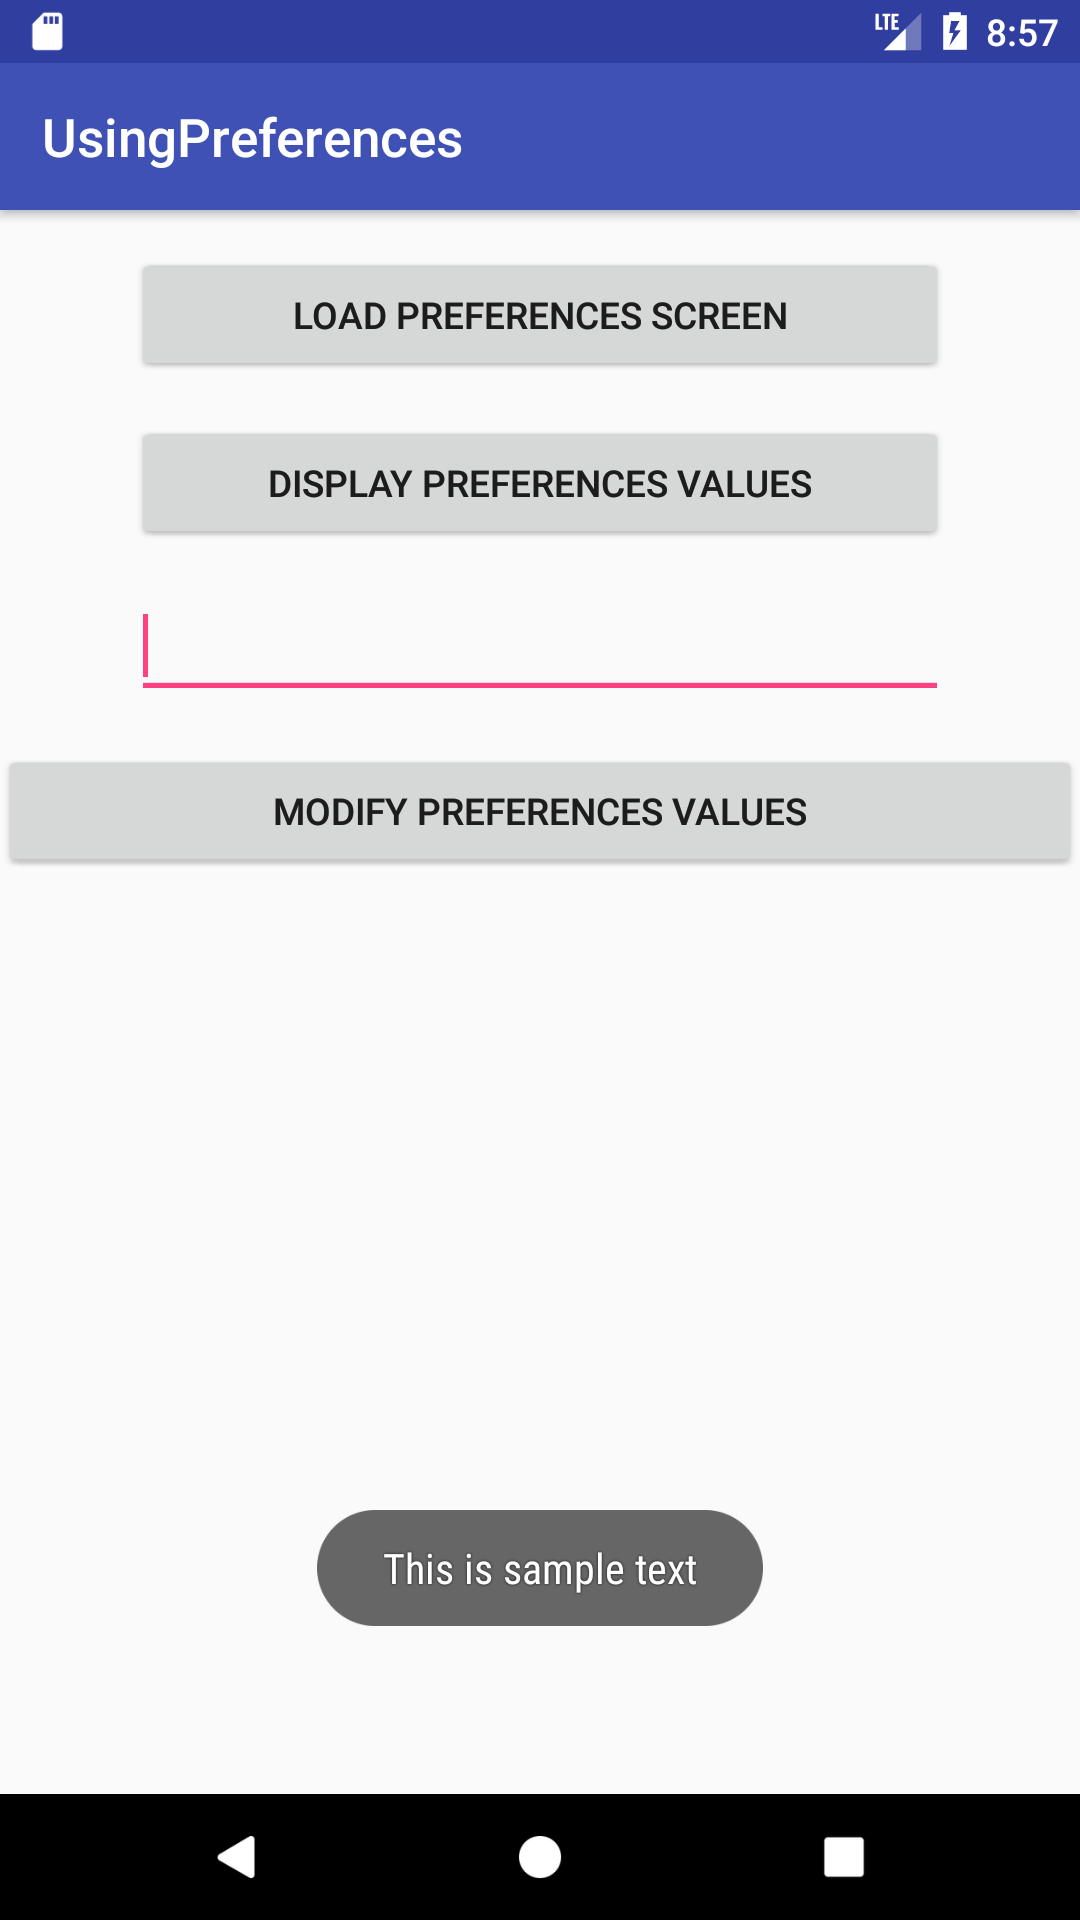
\includegraphics[width=0.7\linewidth]{Screenshot_1497491875}
				\caption{Hasil Akhir (1)}
				\label{fig:screenshot_1497491875}
			\end{minipage}%
			\begin{minipage}{.5\textwidth}
				\centering
				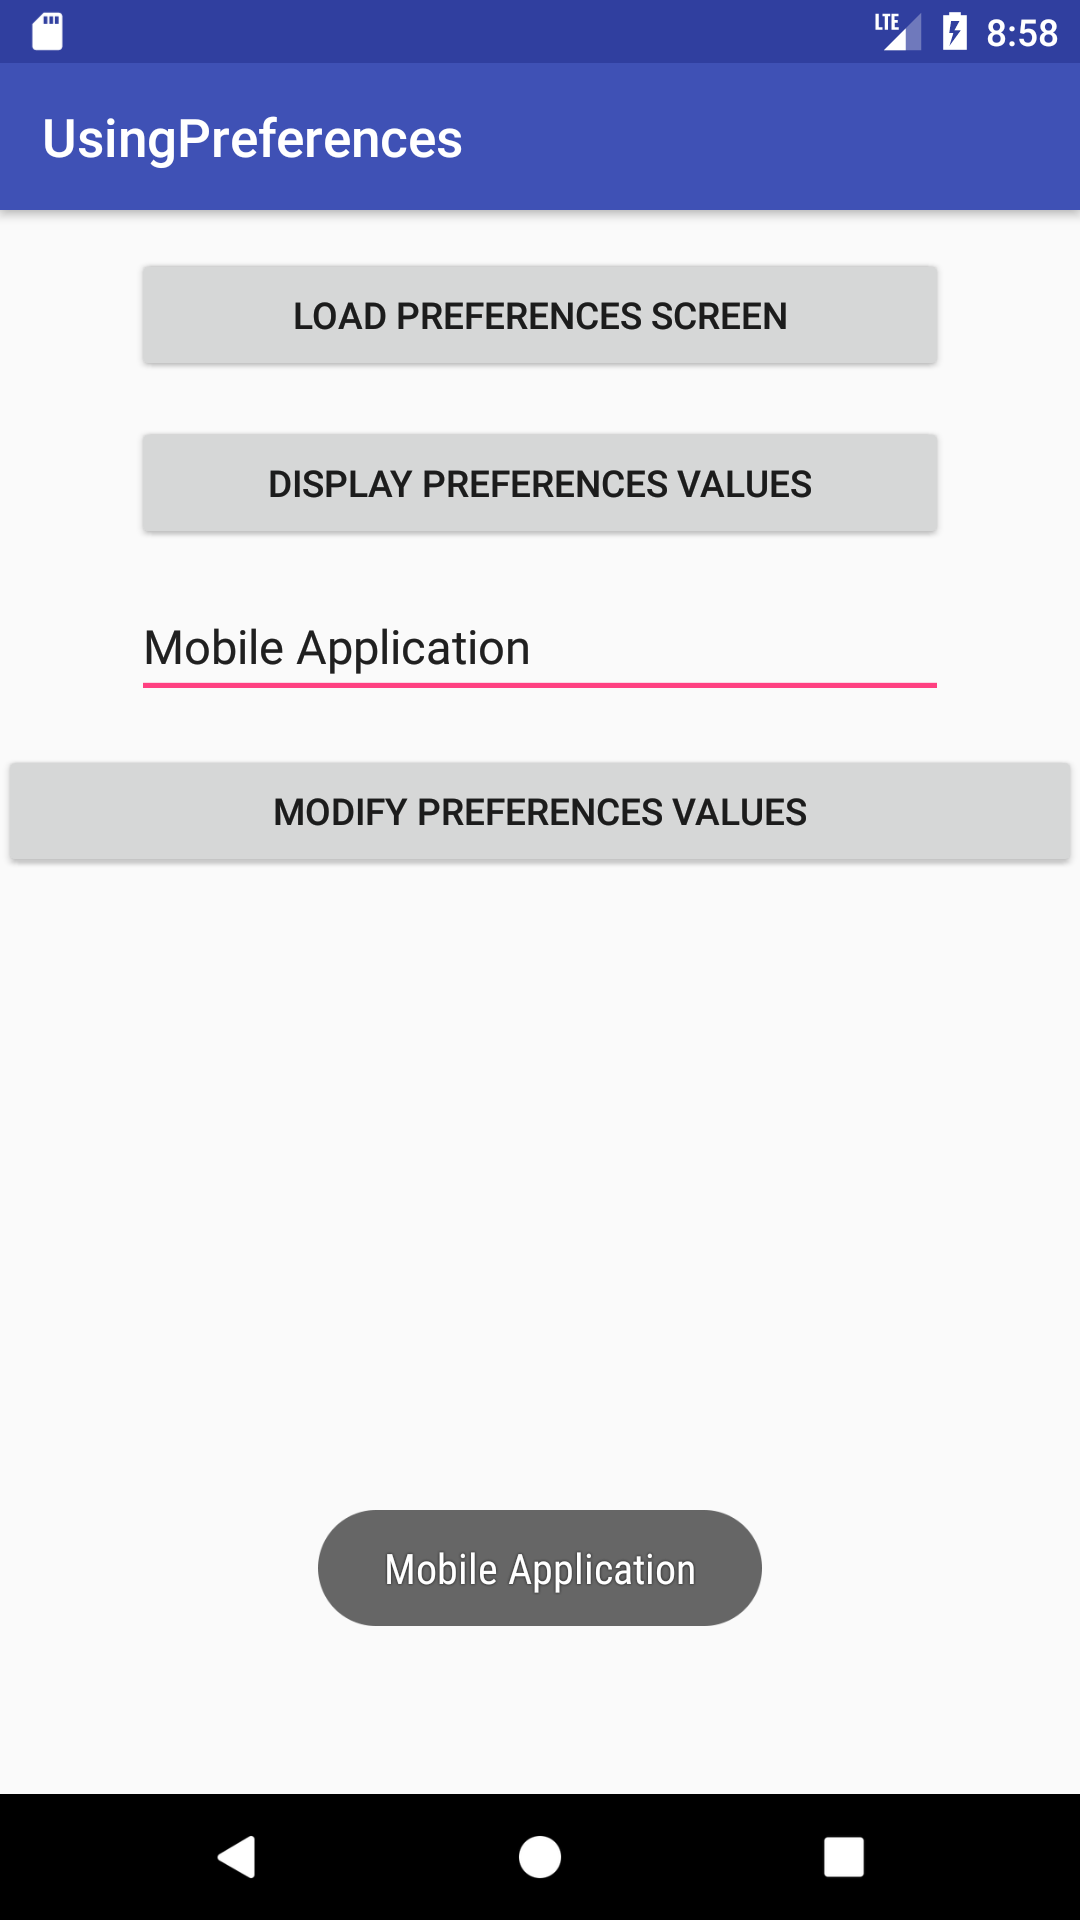
\includegraphics[width=0.7\linewidth]{Screenshot_1497491918}
				\caption{Hasil Akhir (2)}
				\label{fig:screenshot_1497491918}
			\end{minipage}
		\end{figure}
	
		\item Ketik sembarang kalimat pada \texttt{EditText}, lalu klik \texttt{MODIFY PREFERENCES VALUES}.
		
		\item Klik \texttt{DISPLAY PREFERENCES VALUES} untuk memunculkkan nilai \texttt{EditText} yang sudah dimodifikasi sebelumnya (Figur \ref{fig:screenshot_1497491918}).
		
	\end{enumerate}
	
	\subsection{Menyimpan Data ke \textit{Internal Storage}}
	
	\begin{enumerate}
		\item Buat proyek baru dengan nama \textbf{Files} (opsi yang lain dibiarkan \textit{default}).
		\item Buka \texttt{activity\_main.xml}, lalu \textit{copy-paste} listing berikut ini.
		\begin{minted}{xml}
		<?xml version="1.0" encoding="utf-8"?>
			<android.support.constraint.ConstraintLayout xmlns:android="http://schemas.android.com/apk/res/android"
			xmlns:app="http://schemas.android.com/apk/res-auto"
			xmlns:tools="http://schemas.android.com/tools"
			android:id="@+id/activity_main"
			android:layout_width="match_parent"
			android:layout_height="match_parent"
			tools:context="com.example.files.MainActivity">
			
			<TextView
				android:text="Please enter some text."
				android:layout_width="245dp"
				android:layout_height="wrap_content"
				android:id="@+id/textView"
				android:gravity="center"
				app:layout_constraintLeft_toLeftOf="parent"
				app:layout_constraintTop_toTopOf="parent"
				app:layout_constraintRight_toRightOf="parent"
				app:layout_constraintBottom_toTopOf="@+id/editText" />
				
			<EditText
				android:layout_width="241dp"
				android:layout_height="wrap_content"
				android:inputType="text"
				android:ems="10"
				android:id="@+id/editText"
				app:layout_constraintLeft_toLeftOf="parent"
				app:layout_constraintRight_toRightOf="parent"
				app:layout_constraintTop_toBottomOf="@+id/textView"
				app:layout_constraintBottom_toTopOf="@+id/btnLoad" />
			
			<Button
				android:text="Save"
				android:layout_width="240dp"
				android:layout_height="wrap_content"
				android:id="@+id/btnSave"
				app:layout_constraintLeft_toLeftOf="parent"
				app:layout_constraintTop_toBottomOf="@+id/btnLoad"
				app:layout_constraintRight_toRightOf="parent"
				android:onClick="onClickSave"
				app:layout_constraintBottom_toBottomOf="parent" />
				
			<Button
				android:text="Load"
				android:layout_width="241dp"
				android:layout_height="wrap_content"
				android:id="@+id/btnLoad"
				app:layout_constraintLeft_toLeftOf="parent"
				app:layout_constraintTop_toBottomOf="@+id/editText"
				app:layout_constraintRight_toRightOf="parent"
				android:onClick="onClickLoad"
				app:layout_constraintBottom_toTopOf="@+id/btnSave" />
		
		</android.support.constraint.ConstraintLayout>
		\end{minted}
		
		\item Buka file \texttt{MainActivity.java} lalu \textit{copy-paste} listing di bawah ini.
		
		\begin{minted}{java}
		package com.example.files;
		
		import android.support.v7.app.AppCompatActivity;
		import android.os.Bundle;
		import android.view.View;
		import android.widget.EditText;
		import android.widget.Toast;
		
		import java.io.FileInputStream;
		import java.io.FileOutputStream;
		import java.io.IOException;
		import java.io.InputStreamReader;
		import java.io.OutputStreamWriter;
		
		public class MainActivity extends AppCompatActivity {
		
			EditText textBox;
			static final int READ_BLOCK_SIZE = 100;
			
			@Override
			protected void onCreate(Bundle savedInstanceState) {
				super.onCreate(savedInstanceState);
				setContentView(R.layout.activity_main);
				
				textBox = (EditText) findViewById(R.id.editText);
			}
			
			public void onClickSave(View view) {
				String str = textBox.getText().toString();
				try {
					FileOutputStream fOut = openFileOutput("textfile.txt",
							MODE_PRIVATE);
					OutputStreamWriter osw = new OutputStreamWriter(fOut);
				
					// write the string to the file
					try {
						osw.write(str);
					} catch (IOException e) {
						e.printStackTrace();
					}
					osw.flush();
					osw.close();
					
					// display file saved message
					Toast.makeText(getBaseContext(),
							"File saved successfully!", Toast.LENGTH_SHORT).show();
					
					// clears the EditText
					textBox.setText("");
				} catch (IOException ioe) {
					ioe.printStackTrace();
				}
			}
			
			public void onClickLoad(View view) {
				try {
					FileInputStream fIn = openFileInput("textfile.txt");
					InputStreamReader isr = new InputStreamReader(fIn);
					char[] inputBuffer = new char[READ_BLOCK_SIZE];
					String s = "";
					int charRead;
					while ((charRead = isr.read(inputBuffer)) > 0) {
						// convert the chars to a String
						String readString =
						String.copyValueOf(inputBuffer, 0,
						charRead);
						s += readString;
						inputBuffer = new char[READ_BLOCK_SIZE];
					}
				
					// set the EditText to the text that has been read
					textBox.setText(s);
					Toast.makeText(getBaseContext(), "File loaded successfully!",
							Toast.LENGTH_SHORT).show();
				} catch (IOException ioe) {
					ioe.printStackTrace();
				}
			}
		}
		\end{minted}
		
		\item Tekan \texttt{Shift + F9} (atau pilih \texttt{Run > Debug}) untuk men-\textit{debug} aplikasi. Pilih salah satu Android Virtual Device yang kalian inginkan.
		
		\item Ketik sembarang kalimat pada \texttt{EditText} (Figur \ref{fig:screenshot_1497494069}), lalu klik \texttt{SAVE}.
		\begin{figure}[htbp]
			\centering
			\begin{minipage}{.5\textwidth}
				\centering
				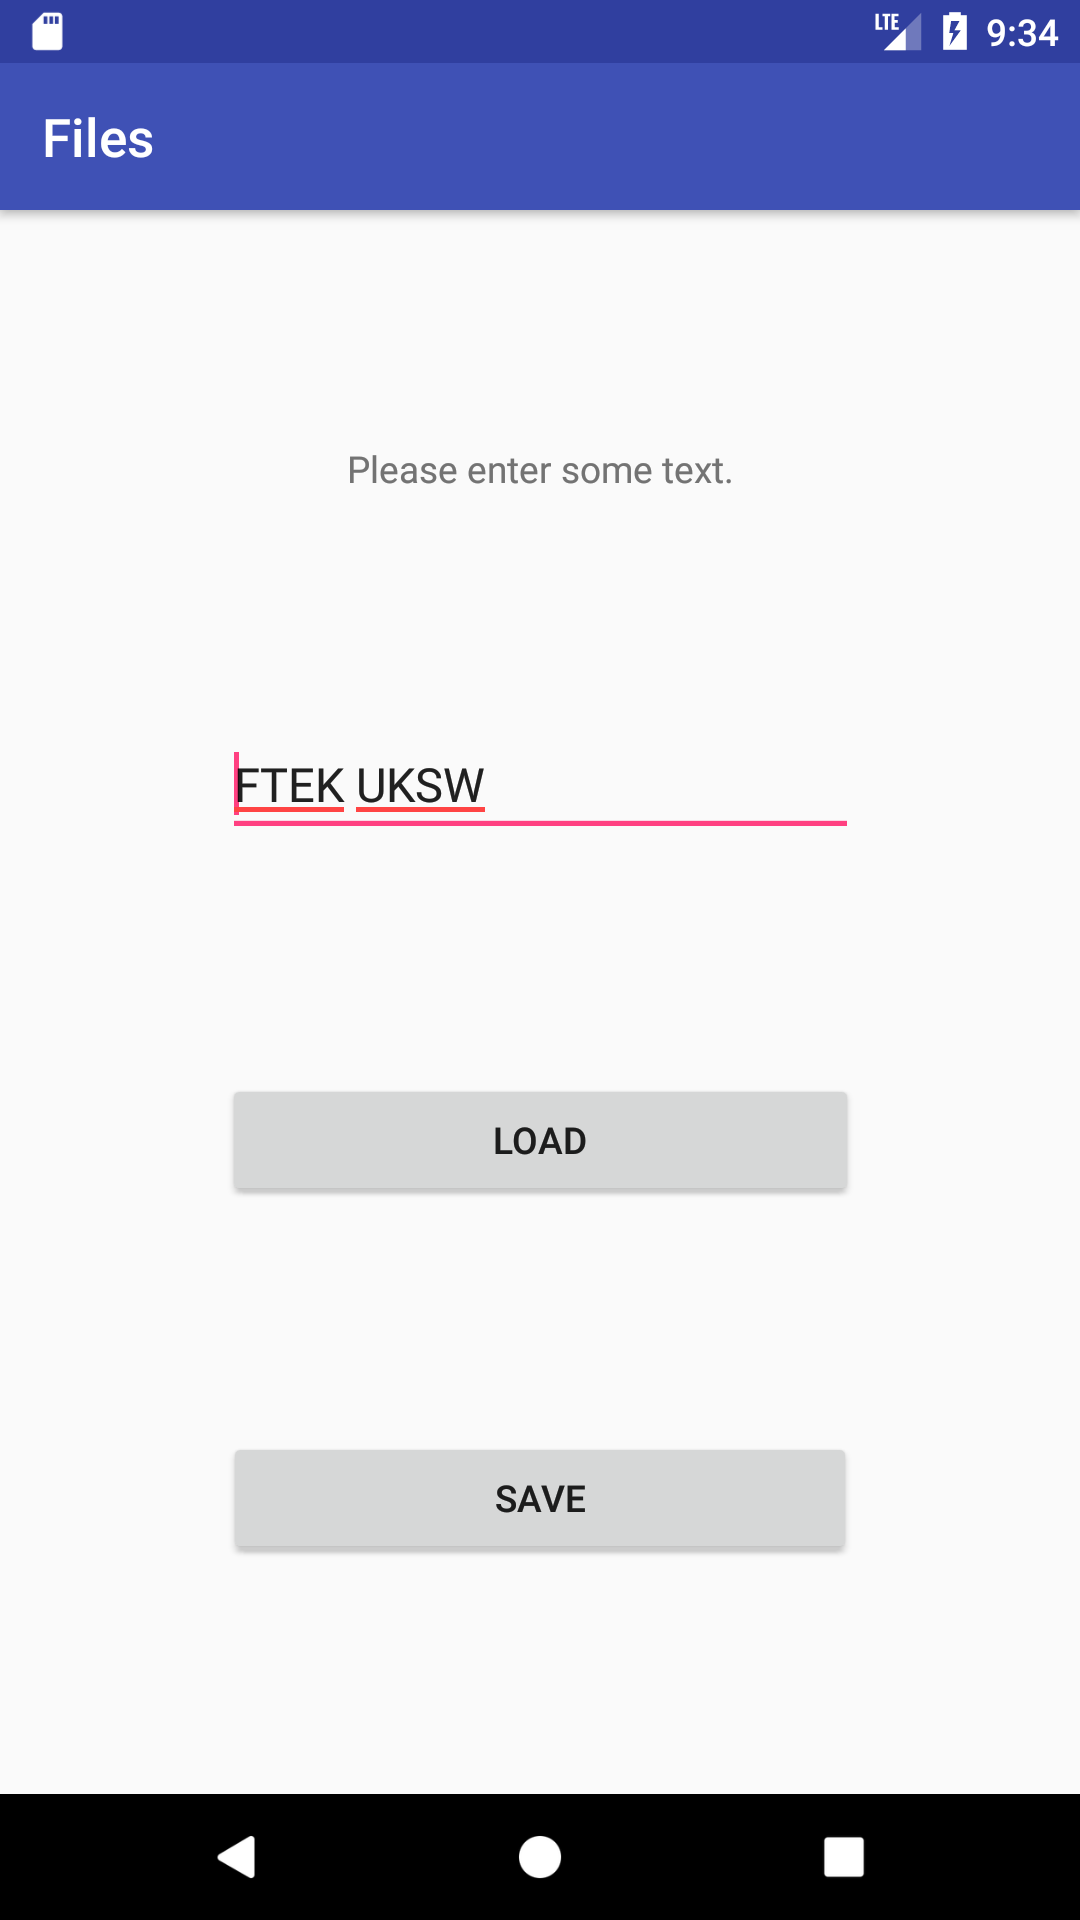
\includegraphics[width=0.7\linewidth]{Screenshot_1497494069}
				\caption{Hasil Akhir (1)}
				\label{fig:screenshot_1497494069}
			\end{minipage}%
		\end{figure}
		\item Jika file sudah disimpan, kalian akan melihat adanya \texttt{Toast} yang menampilkan "File saved successfully!". Teks pada \texttt{EditText} juga menghilang.
		
		\item Klik \texttt{Button} dan kalian akan melihat teks yang barusan kalian simpan. Hal ini menunjukkan bahwa teks sudah tersimpan dengan benar.
		
	\end{enumerate}

	\subsection{Membuat kelas Database Helper}
	
	Pada bagian ini, kita akan membuat basis data dengan nama \texttt{MyDB} yang berisi satu tabel dengan nama \texttt{contacts}. Tabel tersebut memiliki tiga kolom: \texttt{\_id}, \texttt{name}, dan \texttt{email}.
	
	\begin{enumerate}
		\item Buat proyek baru dengan nama \texttt{Databases}.
		
		\item Pilih \texttt{File > New > Java Class} untuk membuat kelas Java baru dengan nama\\ \texttt{DBAdapter}.
		
		\item Buka file \texttt{DBAdapter.java} lalu \textit{copy-paste} listing berikut ini.
		
		\begin{minted}{java}
		package com.example.databases;
		
		import android.content.ContentValues;
		import android.content.Context;
		import android.database.Cursor;
		import android.database.SQLException;
		import android.database.sqlite.SQLiteDatabase;
		import android.database.sqlite.SQLiteOpenHelper;
		import android.util.Log;
		
		public class DBAdapter {
			static final String KEY_ROWID = "_id";
			static final String KEY_NAME = "name";
			static final String KEY_EMAIL = "email";
			static final String TAG = "DBAdapter";
			static final String DATABASE_NAME = "MyDB";
			static final String DATABASE_TABLE = "contacts";
			static final int DATABASE_VERSION = 1;
			static final String DATABASE_CREATE =
					"create table contacts (_id integer primary key autoincrement, "
							+ "name text not null, email text not null);";
			final Context context;
			DatabaseHelper DBHelper;
			SQLiteDatabase db;
			
			public DBAdapter(Context ctx)
			{
				this.context = ctx;
				DBHelper = new DatabaseHelper(context);
			}
			
			private static class DatabaseHelper extends SQLiteOpenHelper
			{
				DatabaseHelper(Context context)
				{
					super(context, DATABASE_NAME, null, DATABASE_VERSION);
				}
				@Override
				public void onCreate(SQLiteDatabase db)
				{
					try {
						db.execSQL(DATABASE_CREATE);
					} catch (SQLException e) {
						e.printStackTrace();
					}
				}
				@Override
				public void onUpgrade(SQLiteDatabase db, int oldVersion, int newVersion)
				{
					Log.w(TAG, "Upgrading database from version " + oldVersion + " to "
							+ newVersion + ", which will destroy all old data");
					db.execSQL("DROP TABLE IF EXISTS contacts");
					onCreate(db);
				}
			}
			
			// opens the database
			public DBAdapter open() throws SQLException
			{
				db = DBHelper.getWritableDatabase();
				return this;
			}
			
			// closes the database
			public void close()
			{
				DBHelper.close();
			}
			
			// insert a contact into the database
			public long insertContact(String name, String email)
			{
				ContentValues initialValues = new ContentValues();
				initialValues.put(KEY_NAME, name);
				initialValues.put(KEY_EMAIL, email);
				return db.insert(DATABASE_TABLE, null, initialValues);
			}
			
			// deletes a particular contact
			public boolean deleteContact(long rowId)
			{
				return db.delete(DATABASE_TABLE, KEY_ROWID + "=" + rowId, null) > 0;
			}
			
			// retrieves all the contacts
			public Cursor getAllContacts()
			{
				return db.query(DATABASE_TABLE, new String[] {KEY_ROWID, KEY_NAME,
						KEY_EMAIL}, null, null, null, null, null);
			}
			
			// retrieves a particular contact
			public Cursor getContact(long rowId) throws SQLException
			{
				Cursor mCursor =
						db.query(true, DATABASE_TABLE, new String[] {KEY_ROWID, KEY_NAME, KEY_EMAIL},
								KEY_ROWID + "=" + rowId, null,
								null, null, null, null);
				if (mCursor != null) {
					mCursor.moveToFirst();
				}
				return mCursor;
			}
			
			// updates a contact
			public boolean updateContact(long rowId, String name, String email)
			{
				ContentValues args = new ContentValues();
				args.put(KEY_NAME, name);
				args.put(KEY_EMAIL, email);
				return db.update(DATABASE_TABLE, args, KEY_ROWID + "=" + rowId, null) > 0;
			}
		}
		\end{minted}
	\end{enumerate}
	
	Program ini belum final karena baru menambah kelas \texttt{DBAdapter.java}. Fungsi kelas tersebut adalah untuk mempermudah kita dalam pembuatan basis data pada Android. Bagian berikutnya akan ditunjukkan cara penggunaan kelas tersebut.
	
	\subsection{Menambah Kontak ke Dalam Tabel}
	
	\begin{enumerate}
		\item Buka proyek \textbf{Databases}.
		\item Buka file \texttt{MainActivity.java} lalu \textit{copy-paste} listing berikut ini.
		
		\begin{minted}{java}
		package com.example.user.databases;
		
		import android.support.v7.app.AppCompatActivity;
		import android.os.Bundle;
		
		public class MainActivity extends AppCompatActivity {
		
			@Override
			protected void onCreate(Bundle savedInstanceState) {
				super.onCreate(savedInstanceState);
				setContentView(R.layout.activity_main);
				
				DBAdapter db = new DBAdapter(this);
				
				// add a contact
				db.open();
				long id = db.insertContact("Markus Antoni", "612013041@student.uksw.edu");
				id = db.insertContact("John Doe", "612013099@student.uksw.edu");
				db.close();
			}
		}
		\end{minted}
		\item Tekan \texttt{Shift + F9} (atau pilih \texttt{Run > Debug}) untuk men-\textit{debug} aplikasi. Pilih salah satu Android Virtual Device yang kalian inginkan.
	\end{enumerate}

	\subsection{Mengambil Semua Kontak Dari Tabel}
	
	\begin{enumerate}
		\item Buka proyek \textbf{Databases}.
		\item Buka file \texttt{MainActivity.java} lalu \textit{copy-paste} listing berikut ini.
		\begin{minted}{java}
		package com.example.databases;
		
		import android.database.Cursor;
		import android.support.v7.app.AppCompatActivity;
		import android.os.Bundle;
		import android.widget.Toast;
		
		public class MainActivity extends AppCompatActivity {
		
			@Override
			protected void onCreate(Bundle savedInstanceState) {
				super.onCreate(savedInstanceState);
				setContentView(R.layout.activity_main);
				
				DBAdapter db = new DBAdapter(this);
				
				// add a contact
				db.open();
				long id = db.insertContact("Markus Antoni", "612013041@student.uksw.edu");
				id = db.insertContact("John Doe", "612013099@student.uksw.edu");
				db.close();
				
				// display all contact
				db.open();
				Cursor c = db.getAllContacts();
				if (c.moveToFirst())
				{
					do {
						DisplayContact(c);
					} while (c.moveToNext());
				}
				db.close();
			}
			
			public void DisplayContact(Cursor c)
			{
				Toast.makeText(this,
						"id: " + c.getString(0) + "\n" +
								"Name: " + c.getString(1) + "\n" +
								"Email: " + c.getString(2),
						Toast.LENGTH_LONG).show();
			}
		}
		\end{minted}
		\item Tekan \texttt{Shift + F9} (atau pilih \texttt{Run > Debug}) untuk men-\textit{debug} aplikasi. Pilih salah satu Android Virtual Device yang kalian inginkan.
	\end{enumerate}
	Perhatikan bahwa terdapat duplikasi kontak di situ. Hal ini dikarenakan setiap kali aplikasi berjalan, 2 kontak pasti dibuat.
	\subsection{Mengambil Kontak dari Tabel}
	\begin{enumerate}
		\item Buka proyek \textbf{Databases}.
		\item Buka file \texttt{MainActivity.java} lalu \textit{copy-paste} listing berikut ini.
		\begin{minted}{java}
		package com.example.databases;
		
		import android.database.Cursor;
		import android.support.v7.app.AppCompatActivity;
		import android.os.Bundle;
		import android.widget.Toast;
		
		public class MainActivity extends AppCompatActivity {
			
			@Override
			protected void onCreate(Bundle savedInstanceState) {
				super.onCreate(savedInstanceState);
				setContentView(R.layout.activity_main);
			
				DBAdapter db = new DBAdapter(this);
				/*
				// add a contact
				db.open();
				long id = db.insertContact("Markus Antoni", "612013041@student.uksw.edu");
				id = db.insertContact("John Doe", "612013099@student.uksw.edu");
				db.close();
				
				// display all contact
				db.open();
				Cursor c = db.getAllContacts();
				if (c.moveToFirst())
				{
					do {
						DisplayContact(c);
					} while (c.moveToNext());
				}
				db.close();
				*/
				
				// get a contact
				db.open();
				Cursor c = db.getContact(2);
				if (c.moveToFirst())
					DisplayContact(c);
				else
					Toast.makeText(this, "No contact found", Toast.LENGTH_LONG).show();
				db.close();
			}
			
			public void DisplayContact(Cursor c)
			{
				Toast.makeText(this,
						"id: " + c.getString(0) + "\n" +
								"Name: " + c.getString(1) + "\n" +
								"Email: " + c.getString(2),
						Toast.LENGTH_LONG).show();
			}
		}
		\end{minted}
		\item Tekan \texttt{Shift + F9} (atau pilih \texttt{Run > Debug}) untuk men-\textit{debug} aplikasi. Pilih salah satu Android Virtual Device yang kalian inginkan.
	\end{enumerate}
	Metode \texttt{getContact()} mengambil satu buah kontak menggunakan ID. Hasil yang dikembalikan adalah berupa obyek \texttt{Cursor}.
	
	\subsection{Update Kontak pada Tabel}
	
	\begin{enumerate}
		\item Buka proyek \textbf{Databases}.
		\item Buka file \texttt{MainActivity.java} lalu \textit{copy-paste} listing berikut ini.
		\begin{minted}{java}
		package com.example.databases;
		
		import android.database.Cursor;
		import android.support.v7.app.AppCompatActivity;
		import android.os.Bundle;
		import android.widget.Toast;
		
		public class MainActivity extends AppCompatActivity {
		
			@Override
			protected void onCreate(Bundle savedInstanceState) {
				super.onCreate(savedInstanceState);
				setContentView(R.layout.activity_main);
				
				DBAdapter db = new DBAdapter(this);
				/*
				// add a contact
				db.open();
				long id = db.insertContact("Markus Antoni", "612013041@student.uksw.edu");
				id = db.insertContact("John Doe", "612013099@student.uksw.edu");
				db.close();
				
				// display all contact
				db.open();
				Cursor c = db.getAllContacts();
				if (c.moveToFirst())
				{
					do {
						DisplayContact(c);
					} while (c.moveToNext());
				}
				db.close();
				
				// get a contact
				db.open();
				Cursor c = db.getContact(2);
				if (c.moveToFirst())
					DisplayContact(c);
				else
					Toast.makeText(this, "No contact found", Toast.LENGTH_LONG).show();
				db.close();
				*/
				
				// update contact
				db.open();
				if (db.updateContact(1, "Oscar Diggs", "oscar@oscardiggs.com"))
					Toast.makeText(this, "Update successful.",
							Toast.LENGTH_LONG).show();
				else
					Toast.makeText(this, "Update failed.", Toast.LENGTH_LONG).show();
				db.close();
			}
			
			public void DisplayContact(Cursor c)
			{
				Toast.makeText(this,
						"id: " + c.getString(0) + "\n" +
								"Name: " + c.getString(1) + "\n" +
								"Email: " + c.getString(2),
						Toast.LENGTH_LONG).show();
			}
		}
		\end{minted}
		\item Tekan \texttt{Shift + F9} (atau pilih \texttt{Run > Debug}) untuk men-\textit{debug} aplikasi. Pilih salah satu Android Virtual Device yang kalian inginkan.
	\end{enumerate}
	Metode \texttt{updateContact()} digunakan untuk meng-\textit{update} kontak sebelumnya. Dalam contoh ID 1 yang sebelumnya berisi kontak "Markus Antoni" telah diganti menjadi "Oscarr Diggs". Hasilnya adalah sebuah nilai Boolean yang menandakan apakah \textit{update} tersebut berhasil dilakukan atau tidak.
	
	\subsection{Menghapus Kontak dalam Tabel}
	
	\begin{enumerate}
		\item Buka proyek \textbf{Databases}.
		\item Buka file \texttt{MainActivity.java} lalu \textit{copy-paste} listing berikut ini.
		\begin{minted}{java}
		package com.example.databases;
		
		import android.database.Cursor;
		import android.support.v7.app.AppCompatActivity;
		import android.os.Bundle;
		import android.widget.Toast;
		
		public class MainActivity extends AppCompatActivity {
		
			@Override
			protected void onCreate(Bundle savedInstanceState) {
				super.onCreate(savedInstanceState);
				setContentView(R.layout.activity_main);
				
				DBAdapter db = new DBAdapter(this);
				/*
				// add a contact
				db.open();
				long id = db.insertContact("Markus Antoni", "612013041@student.uksw.edu");
				id = db.insertContact("John Doe", "612013099@student.uksw.edu");
				db.close();
				
				// display all contact
				db.open();
				Cursor c = db.getAllContacts();
				if (c.moveToFirst())
				{
					do {
						DisplayContact(c);
					} while (c.moveToNext());
				}
				db.close();
				
				// get a contact
				db.open();
				Cursor c = db.getContact(2);
				if (c.moveToFirst())
					DisplayContact(c);
				else
					Toast.makeText(this, "No contact found", Toast.LENGTH_LONG).show();
				db.close();
				
				// update contact
				db.open();
				if (db.updateContact(1, "Oscar Diggs", "oscar@oscardiggs.com"))
					Toast.makeText(this, "Update successful.",
						Toast.LENGTH_LONG).show();
				else
					Toast.makeText(this, "Update failed.", Toast.LENGTH_LONG).show();
				db.close();
				*/
				
				// delete a contact
				db.open();
				if (db.deleteContact(1))
					Toast.makeText(this, "Delete successful.",
							Toast.LENGTH_LONG).show();
				else
					Toast.makeText(this, "Delete failed.", Toast.LENGTH_LONG).show();
				db.close();
			}
			
			public void DisplayContact(Cursor c)
			{
			Toast.makeText(this,
					"id: " + c.getString(0) + "\n" +
							"Name: " + c.getString(1) + "\n" +
							"Email: " + c.getString(2),
					Toast.LENGTH_LONG).show();
			}
		}
		\end{minted}
		Metode \texttt{deleteContact()} digunakan untuk menghapus kontak pada tabel yang sebelumnya sudah dibuat. Hasilnya adalah sebuah nilai Boolean yang menandakan apakah kontak tersebut berhasil dihapus atau tidak.
		
	\end{enumerate}

	\vspace*{\fill}
	\begin{center}
		\large{\textbf{THE END}}
	\end{center}
	
\end{document}